\subsection{Why does bureaucracy exist? Can't we just do the work?\label{sec:alternatives_to_bureaucracy}}

In this section we'll explore a few alternatives to bureaucracy. 



% https://graphthinking.blogspot.com/2021/02/how-to-have-efficient-bureaucracy.html

\subsubsection{Efficient Bureaucracy}

In an ideal scenario with no bureaucracy, everyone comes to the same conclusion when presented with the same information. Then the management process of building consensus becomes unnecessary. There is no need to fight over resources (money, staffing) and no need to fight over direction.

While that ideal scenario is not going to happen, it points to how to improve bureaucratic efficiency:
\begin{itemize}
\item each person has the same information. 
\item each person applies the same decision making process consistently
\item every person has the same incentives
\end{itemize}
The reason bureaucracy is inefficient is
\begin{itemize}
    \item not everyone has the same information
    \item processes are inconsistent
    \item incentives vary
% https://graphthinking.blogspot.com/2017/03/what-slows-down-bureaucracy.html
    \item Imprecise language
    \item Using opinions and experience rather than collect data and analyze data
    \item prioritizing by putting out fires rather than attacking largest issues
    \item not responding to communications (email, phone, meetings)
    \item being late to meetings
    \item scope creep
    \item planned scope and capability scope (due to staffing or skills) is mismatched
    \item silos of operation
% https://graphthinking.blogspot.com/2017/03/progress-in-spite-of-better-ways.html
    \item lies
    \item mistakes
\end{itemize}
Also, add the issue that each person's reference experiences are unique. As a consequence, decision making is subjective. 




\subsubsection{Perfect bureaucracy}

Starting with ``perfect bureaucracy'', there are two perspectives: that of the subject and that of the bureaucrat. 

From the perspective of the subject of a bureaucratic organization, perfect bureaucracy means minimizing the time the subject waits on a decision, and means getting perfectly correct decisions, decisions are consistent across subjects and circumstances, decisions take into account all relevant factors, and there is zero cost to the subject. Any process deviating from those expectations is a noticble detriment to the subject, leading to the negative reference experiences of bureaucracy. Nevermind that the desires are unreasonable and conflicting. In a real bureaucracy, subjects have a negative or neutral experience, with rare positive interactions.

Perfect bureaucracy for a bureaucrat means all information is available, information is immediately available, and there is no moral ambiguity (answer is objective). Trade-offs become trivial and the emotional toll of the work goes to zero. Then the bureaucrat is able to serve subjects (an emotionally rewarding prospect). Note that this job might be feel hollow if all decisions are obvious. In a real bureaucracy, the typical experience is negative or neutral, punctuated by glimpses of satisfaction. 

\subsubsection{Everyone do their own thing -- No coordination, No bureaucracy}
The minimal scenario to start from is to imagine a single person working on a single task that does not last long (a few minutes), is relatively easy (cognitively and physically and emotionally), and does not recur. In that situation, building consensus is irrelevant and no process is required. Even then, it is often the case that this simple task involves the use of shared limited resources -- basic essentials like water, air, land. If you task involves use of those things, then how is equitable use determined among consumers?

Even for simplistic tasks, the concept of self-serve shared resources for each person is not trivial. independent allocation of shared resources breaks down and access is determined by violence.

Most of what you do occurs beyond the limits of simplicity and thus incurs some concept of \gls{process} (breaking a task into subtasks). Staying with the one-person constraint, a complex task can benefit from being broken into subtasks. Sometimes the order of the subtasks matters, so we need to track the dependencies. A recurring multi-step process with documentation is starting to have features of bureaucracy, but lacks the need for consensus. 


If one person lacks the skills relevant to a multi-step process, they may engage another person to help. The interaction may be informal (anarchy) or formalized in a contract (\href{https://en.wikipedia.org/wiki/Libertarianism}{libertarian}). If the parties working on the task fail to reach consensus, what is the recourse? Options include physical violence, threats, or involving a third party (e.g., a court with lawyers and judges). 


To summarize, two aspects necessitate bureaucracy: shared resources and shared responsibility. 
If you want to manage resources and responsibilities, how is that policy decided?  Building consensus is relevant, but what is the process for establishing consensus?

Nepotism and cultural norms and religious practices served this role prior to bureaucracy. 


\subsubsection{limit bureaucracy to a single decider}
If we are going to live in a society, what if we had a single person deciding?

how fast could that be?

Good decisions can't be instantaneous -- the OODA cycle is necessary.

If OODA takes X minutes, then in a 10 hour work day that's a max of 600/X decisions.



Monarchies and dictatorships the rely on a single decider. A simpler model to understand, but difficult to handle all the edge cases for large society. A single decider doesn't scale for the number of decisions needed, so the decider then appoints bureaucrats to subjectively implement policies. 


perfect bureaucracy of one person doesn't scale. Can't say "just automate everything" because carrying out the approach requires a staff to implement. Automation isn't free -- it requires creation and maintenance

\subsubsection{automation of processes}

The role of automation is to make interactions more predictable, faster, scalable,

% https://graphthinking.blogspot.com/2019/07/bureaucracy-is-social-process-executed.html
when to transition a human-based bureaucratic process to automation:
* Stability of process
* Expected lifespan of need for process; how long until it is displaced?
* availability of objective evaluation criteria for business logic
* frequency of recurrence
* cost of automating (NRE+OandM)
% https://graphthinking.blogspot.com/2019/07/cost-of-creating-and-supporting.html
\footnote{https://xkcd.com/1319/ and https://xkcd.com/1205/}


\subsubsection{complexities of more than one bureaucrat}

% https://graphthinking.blogspot.com/2019/07/first-principles-analysis-of-creating.html

If there's more than one person, then communication for consensus takes time (the "observe/orient" phases) and decreases the decision throughput

perfect bureaucracy requires everyone know everyone else's job skills and responsibilities

would perfect bureaucracy involve ``everyone has the same view" or ``there is a diversity of views that enable robustness"?



\textbf{Elected representatives}\\
Political representatives are an easier to understand concept because it's just one person acting in that behalf of other people.
In contrast emergent behavior of bureaucracy is more difficult to understand. 
TODO: why not make the entire system out of politicians?


TODO: thought experiment: 
What if everybody in a bureaucracy were the same?
What if everybody in a bureaucracy had a different opinion?


If you think bureaucracy sucks and it should be removed or replaced, then the parable of Chesterton's fence applies. Understanding not the history of the bureaucracy, but the reason it exists

\begin{quote}
There exists ... a fence or gate erected across a road. The more modern type of reformer goes gaily up to it and says, “I don’t see the use of this; let us clear it away.” To which the more intelligent type of reformer will do well to answer: “If you don’t see the use of it, I certainly won’t let you clear it away. Go away and think. Then, when you can come back and tell me that you do see the use of it, I may allow you to destroy it.\footnote{``The Thing'' (1929) Chesterton, in the chapter, “The Drift from Domesticity”; https://www.chesterton.org/taking-a-fence-down/}
\end{quote}

Suppose that you don't have oversight of your processes in your finances and your resources. A small percentage of the population say 0.1\%, will take advantage of that lack of a per side for their own game. Those malicious actors show as subjects of bureaucracy and as bureaucrats within the organization. 
\cite{2012_Schneier} calls these defectors



The short answer is that bureaucracy is a response to the complexity of a problem being solved. To see why that is, let's start simple and then increase the complexity. 



The bureaucrat's identity is subsumed into service for the organization they are part of. At the same time, bureaucracy enables the bureaucrat to amplify their presence by being part of a larger organization. A bureaucrat can accomplish more as part of an organization than by working alone. Sometimes the cost of being part of the organization exceeds the force multiplier of working together. 

% https://graphthinking.blogspot.com/2021/09/why-is-everything-so-hard-in-large.html

What if we completely avoided bureaucracy? That question is better worded by replacing ``bureaucracy" with ``coordination of stakeholders". If you avoid coordination of stakeholders, you either are constrained to only work on tasks that involve one person, or you get is random (uncoordinated) interactions. 

What if we minimized bureaucracy? Again, try replacing ``bureaucracy" in that question with ``coordination of stakeholders". The goal of ``minimizing coordination" probably isn't the real objective. To be more precise, a specific objective might be ``minimize time spent executing the task" (which takes a lot of coordination prior to the task execution) or ``minimize the level of distraction to stakeholders" (chunk the coordination time). Another strategy for minimizing bureaucracy is to reduce the number of stakeholders involved. For a given task complexity, this means having smarter people who have more skills. 

\begin{figure}
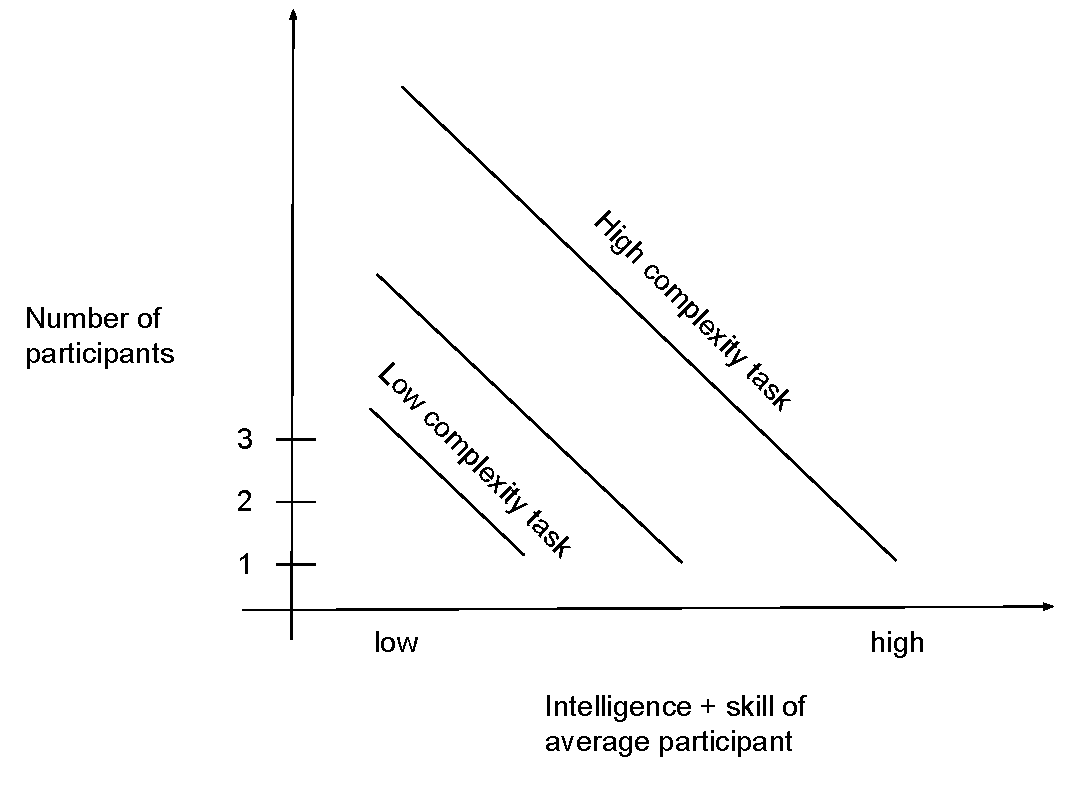
\includegraphics[width=0.8\textwidth]{images/people-per-task-for-skill-level.pdf}
\caption{Three levels of task complexity are shown. As task complexity increases, the size of the team needs to grow. The growth may be less if the team members are brilliant. Those brilliant people cost more and there are fewer of them available.}
\end{figure}
